\documentclass{article}
\usepackage{nips15submit_e,times}
\usepackage{hyperref}
\usepackage{url}

\usepackage[table]{xcolor}
\usepackage{colortbl}
\usepackage{graphicx}
\usepackage[normalem]{ulem}


\title{Towards Distributed, Asynchronous Reinforcement Learning on Consumer Compute}


\author{
Gordon Chen\\
School of Computing\\
University of Connecticut\\
\texttt{gbc24001@uconn.edu}\\
}

\newcommand{\fix}{\marginpar{FIX}}
\newcommand{\new}{\marginpar{NEW}}

\nipsfinalcopy

\begin{document}


\maketitle

\begin{abstract}
Deep learning research increasingly depends on access to large amounts of compute. At the same time,
due to recent interest in deep learning, compute is becoming harder to access for student researchers
and hobbyists.
In this project, we experiment with building a distributed, asynchronous reinforcement learning protocol
that can make use of idle consumer compute over the internet.
Building off of existing distributed, asynchronous reinforcement learning algorithms like IMPALA and IMPACT,
this project aims to explore the algorithmic and engineering challenges in making it work, attempt
improvements such as reducing communication overhead via trajectory compression, and create a flexible
framework for students and researchers to use for consumer compute pooling.
\end{abstract}


\section{Problem}
Due to the increased interest in deep learning, compute for student and hobbyist research is becoming harder
to access. Both memory and GPUs are getting more expensive, and cloud compute providers frequently run out of
GPU instances when demand is high. Models are getting bigger and experiments are getting more expensive,
meaning that even relatively small research projects can be constrained by access to compute.

Simultaneously, a large amount of consumer compute, such as desktops and gaming PCs,
sits around unused for most of the day. Many students and hobbyists often have desktops with decent hardware
that spend much of the day idle, because alone, these machines are often not powerful enough individually
for larger modern deep learning experiments, even though collectively they may represent a substantial pool
of useful compute.


\section{Goal}
The goal of this project is to build a distributed, asynchronous reinforcement learning protocol that
allows multiple geographically scattered machines to contribute compute to a shared training run
over the internet.
The protocol would follow the setup from IMPALA, with actor nodes that collect trajectories using local,
possibly stale, copies of the policy, and periodically send those trajectories to a central learner
over the internet, and receive updated model parameters in return.
Rather than attempting to build a complete production-quality protocol,
this project aims to see how realistic this idea is at all: if distributed, asynchronous reinforcement
learning can make effective use of this kind of compute in a practical way, even over the internet,
despite stale policies, communication overhead, and heterogeneity in machine performance.

The motivating use case is something like a group of students agreeing to let each other borrow compute
from each other's idle desktops to perform RL research none of them would have the computing resources to
do alone. This project seeks to build a flexible protocol that makes this kind of compute pooling work,
making it easy for students to share compute and tackle larger projects.


\section{Importance}
This is an important project because access to compute is a major bottleneck for students who want to do
deep learning research. As models and experiments become more expensive, the barrier to entry keeps rising.
This affects education directly, because students with limited funding are forced to choose smaller and less
ambitious projects, not because the ideas are bad, but because the compute is unavailable.

I think there is a real opportunity here to democratize reinforcement learning research by making it easier
to use compute that already exists but is idle. If distributed, asynchronous RL can be made practical on
existing consumer hardware over the internet, then students could potentially collaborate by
sharing spare compute instead of each person needing their own expensive training setup.

Furthermore, there is quite a bit of difference between the homogenous, within-datacenter, distributed
training that IMPALA was meant for, and the heterogeneous, unreliable, bandwidth-limited situation of
compute pooling over the internet that this project is meant to target.


\section{Algorithms}
For the actual reinforcement learning algorithm, I plan to start by using IMPALA and V-trace, since
IMPALA is explicitly designed for distributed, asynchronous RL with stale policies.
If time permits, I would also like to explore IMPACT, a work that builds on IMPALA's V-trace, and compare them
to see if IMPACT can perform better than IMPALA in this setting. IMPALA has multiple actor nodes that roll out
trajectories with a local, possibly stale, actor. The actor nodes send trajectories to the learner, which
uses policy gradients with V-trace importance sampling corrections to learn from those trajectories, and then
sends back the updated weights to the workers.

In IMPALA, actor nodes must send full trajectories to the learner node. Since internet bandwidth
strongly constrains the speed at which trajectories can be transferred to the learner, one way I will attempt
to improve IMPALA is through trajectory compression. If I could compress trajectories on the actor, send much
smaller trajectories to the learner, and then reconstruct the full trajectories on the learner, then I could
save quite a bit of slow cross-internet data transfer. I will first start with classical lossless compression
algorithms such as frame differencing or delta encoding to compress Atari frames. If time permits I would also
like to experiment with learned compression methods such as using a pretrained VAE, or even training the VAE
jointly with the RL system. Since I want this protocol to be general enough for different RL
problems and not tied to a single environment, I think my protocol will have an optional compression and
reconstruction stage that the protocol users can implement if they want.


\section{Data}
I plan to start with classic RL environments such as Atari games. Atari is a good place for me to start
because it is a well known environment that many people have already benchmarked their algorithms on,
which will serve as a good comparison point for my new protocol. Furthermore, it is complex enough that
some RL algorithm implementations can take a very long time to train on it.

Since I want to make a general protocol for distributed, async RL, I plan to get my protocol working on at least
2 Atari environments to demonstrate that the protocol is a flexible framework that can support many environments.

If time permits, I may explore other RL tasks that are well suited to asynchronous distributed training.
One possibility would be reinforcement learning for language models, but I think it is much more important
that I first get the protocol working reliably on Atari or other standard RL tasks. However, in the long term,
I would like to get RL fine tuning working for LLMs because the potentially long reasoning rollouts are, in my
opinion, well suited for asynchronous RL, and the large computational requirements for LLM fine-tuning make
this problem attractive for compute-pooling and democratization.


\section{Expected Results}
The ultimate goal of this project is to have my distributed protocol train faster (reach a fixed
target reward faster in wall-clock time) compared to a strong synchronous baseline (probably PPO)
on a single machine.
However, for relatively small RL problems like Atari
the bandwidth overhead may outweigh the speedup from parallelization on many machines and this may not
be possible. I might then need to experiment with harder environments that require larger models, which
should benefit from parallelization more than PPO which already fits on a single machine easily.

Furthermore, I want to demonstrate that it is possible to implement a practical distributed async RL
protocol despite problems of stale policies, internet communication, and heterogeneous compute capabilities.
I also hope to identify the best algorithm for this task, if IMPACT can outperform IMPALA, and if I can find
anything to make better in those existing algorithms.
I also want to experiment with trajectory compression, and see if it can reduce internet communication
bandwidth and speed up training. Even negative results would be useful here, since they would show what makes
distributed async RL on heterogeneous consumer compute difficult in practice.

If all goes well, I would also like to show that the protocol is not tied to a single game by evaluating it
on more than one environment. This would support the claim that the framework is flexible enough to be useful
for reinforcement learning research more generally.


\section{Progress}
So far, I have written a strong PPO baseline for Pong (Figure \ref{fig:pong_ppo}) that I can use to
benchmark my distributed RL protocol against. This gives me a reference point for both sample
efficiency and training speed.

\begin{figure}[h]
    \centering
    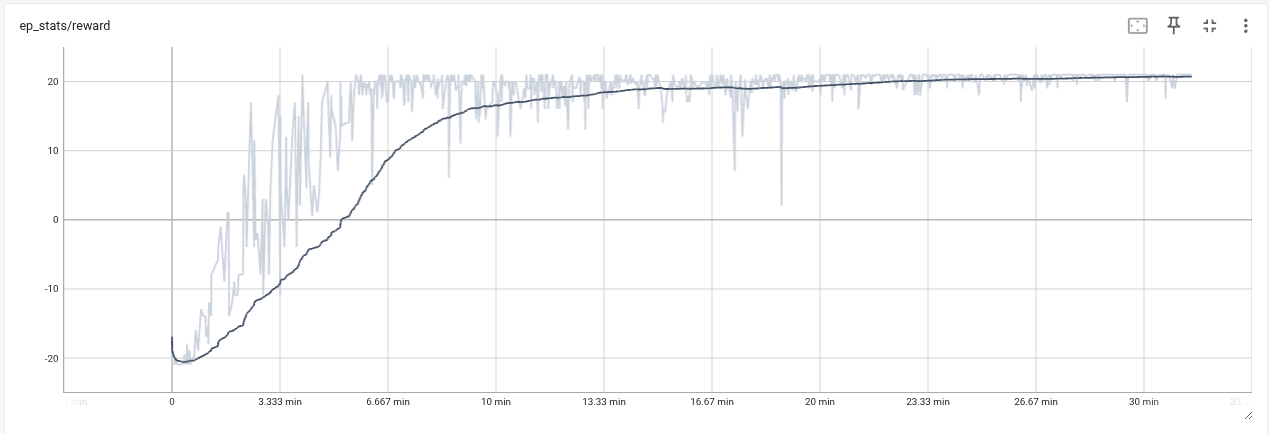
\includegraphics[width=\textwidth]{midpt_imgs/pong_ppo.png}
    \caption{Pong PPO baseline.}
    \label{fig:pong_ppo}
\end{figure}

I spent a long time looking through the distributed RL literature and found that IMPALA and IMPACT were the
SOTA algorithms. I have fully read the IMPALA paper now, and have worked through the math
and now understand what it does and why. I implemented a synchronous version of IMPALA with V-trace importance
sampling correction on Pong (Figure \ref{fig:pong_impala_sync}).
This is a good starting point for me to start moving to the distributed and
asynchronous parts now that I have the critical IMPALA V-trace algorithm down.

\begin{figure}[h]
    \centering
    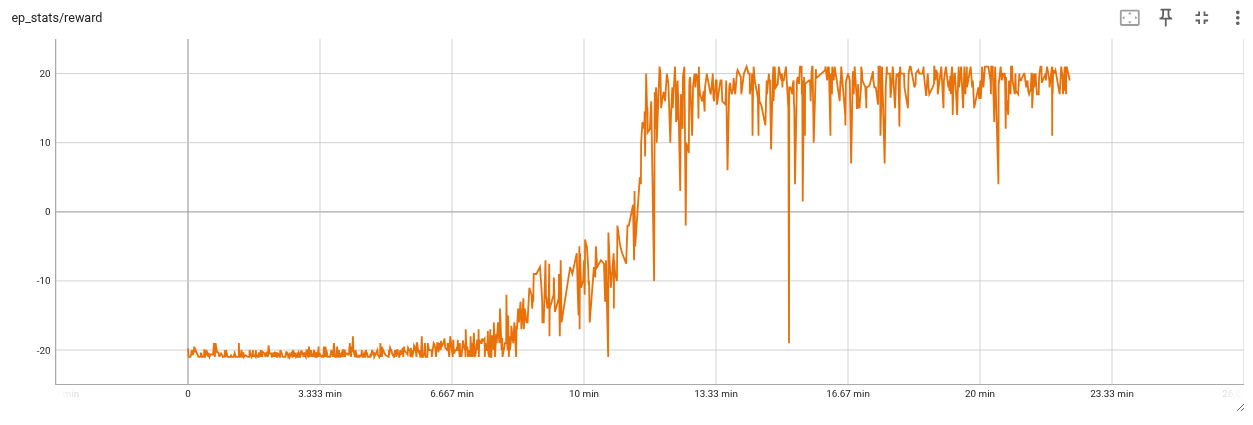
\includegraphics[width=\textwidth]{midpt_imgs/pong_impala_sync.png}
    \caption{Pong Synchronous IMPALA.}
    \label{fig:pong_impala_sync}
\end{figure}


\section{Issues + Plans to Fix}
One issue that I am currently seeing is that IMPALA is less sample-efficient than PPO. My IMPALA takes roughly
2 times more epochs than PPO to consistently reach 21 reward on Pong. This also makes it slower in wall
clock time to reach 21 reward, which is bad because the whole point of this project was to do async RL training
faster than sync. Furthermore, I already did a rough learning rate sweep for IMPALA to see if that would make
it converge as fast as PPO but it just doesn't, so the issue is unlikely to be hyperparameter tuning related
and more likely just an algorithmic sample efficiency limitation.

I plan to fix this by trying out IMPACT (which is also sometimes called Asynchronous PPO) because IMPACT
claims to match PPO's sample-efficiency. So later I will read, implement, and benchmark IMPACT to see if it
performs better than IMPALA and if it actually is as sample-efficient as advertised.

The larger problem with what I have right now is that I currently only have synchronous IMPALA implemented.
While understanding and implementing IMPALA's V-trace importance sampling correction is a very important
part of this project, inspecting IMPALA's importance sampling weights, they are all so close to $1$ because
I am running synchronously so I'm not even really stress-testing IMPALA's off-policy correction.

I plan to fix this by having the next thing I work on be splitting my synchronous IMPALA training code
into asynchronous learner and actor programs. That way I can run IMPALA asynchronously, just by having 2
processes on a single machine first. Then I'll have a circular trajectory buffer on the learner so I'll be
able to stress-test IMPALA with actually stale policies and see how much performance degradation there is.
This is also when I'll start experimenting with trajectory compression. It will be much more necessary
for when the learner and actor are distributed across different devices and the internet communication
bandwidth comes into play.

After I have a learner and actor running asynchronously on different processes on a single device, the next
step will be to figure out the networking I will need to have the learner and actor on different devices,
communicating over the internet.

At this point I'll then just try my protocol on different envs to demonstrate its flexibility, and start
looking into where I can squeeze out more performance from my protocol so that I can beat synchronous PPO.


\section{Schedule}

\renewcommand{\arraystretch}{1.2}
\begin{tabular}{ |l|l|l| }
 \hline
 Week of 4/10 & \cellcolor{red} Midpoint check & PPO baseline + Synchronous IMPALA.\\
 \hline
 Week of 4/17 & & Asynchronous IMPALA + Trajectory compression.\\
 \hline
 Week of 4/24 & & Distributed Async IMPALA + Work on presentation.\\
 \hline

 4/23 - 4/30 & \cellcolor{red} Presentation & 15-min presentation: problem formulation, algs, results, demo \\
 \hline

 Week of 5/1 & & IMPALA vs IMPACT, 2nd env. Work on final report\\
 \hline
 Week of 5/8 & & $\downarrow$\\
 \hline

 5/8 & \cellcolor{red} Final report & 6-page report: problem formulation, algs, results. \\
 \hline
\end{tabular}

% \subsubsection*{Acknowledgments}
% \subsubsection*{References}
\end{document}
